\begin{figure}[h]
    \centering
    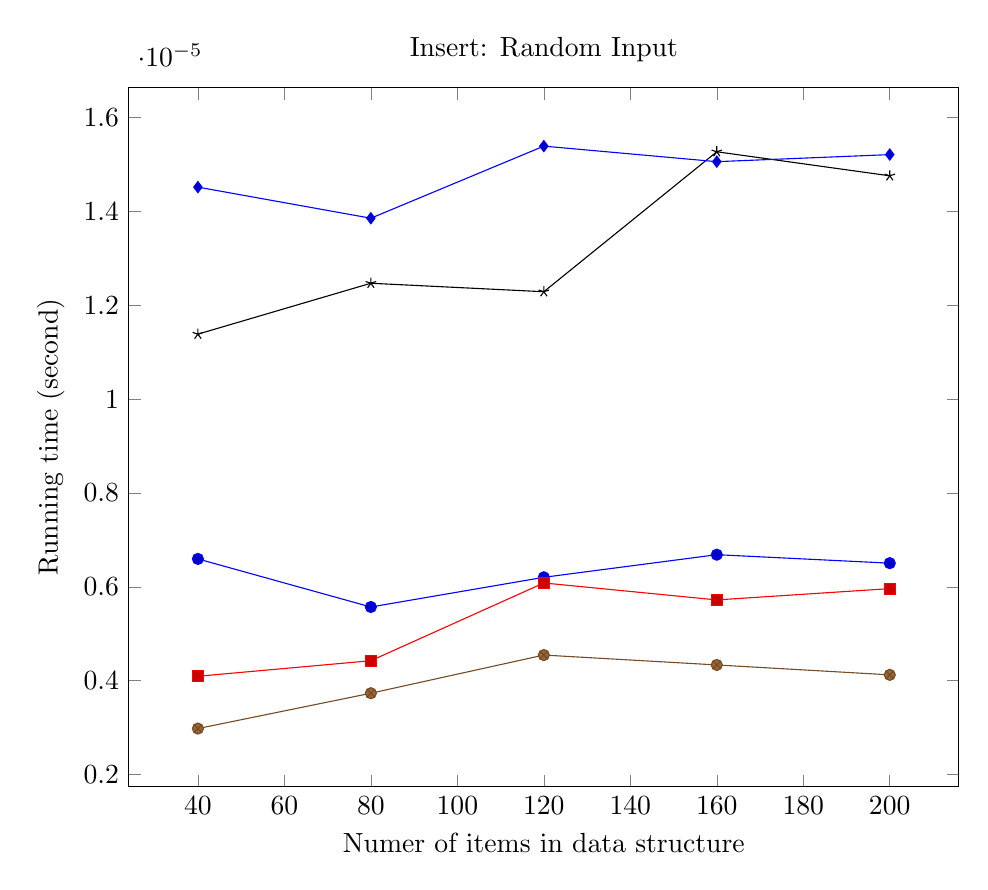
\begin{tikzpicture}
        \begin{axis}[
            xlabel={Numer of items in data structure},
            ylabel={Running time (second)},
            title={Insert: Random Input},
            width=\textwidth
        ]
		\addplot coordinates {
			(200, 6.505387273847419e-06)
			(160, 6.686092475760575e-06)
			(120, 6.204211937088644e-06)
			(80, 5.57174372985969e-06)
			(40, 6.59573987462636e-06)
		};
		\addplot coordinates {
			(200, 5.9632716677526785e-06)
			(160, 5.722331398416713e-06)
			(120, 6.083741802243025e-06)
			(80, 4.427277450247402e-06)
			(40, 4.095984579777223e-06)
		};
		\addplot coordinates {
			(200, 4.126102113488628e-06)
			(160, 4.33692484946846e-06)
			(120, 4.547747584737749e-06)
			(80, 3.734574175950911e-06)
			(40, 2.9816358338763393e-06)
		};
		\addplot coordinates {
			(200, 1.4757591500824674e-05)
			(160, 1.526958957320801e-05)
			(120, 1.228795373933167e-05)
			(80, 1.2468658941600096e-05)
			(40, 1.1384427729055347e-05)
		};
		\addplot coordinates {
			(200, 1.52093545057852e-05)
			(160, 1.5058766837583449e-05)
			(120, 1.5390059708053626e-05)
			(80, 1.3854065490548351e-05)
			(40, 1.451665123148871e-05)
		};
        \legend{}
        \end{axis}
    \end{tikzpicture}
    \caption{Average of 0 operations, benchmarked every 0, starting at 0.}
\end{figure}